\documentclass[10pt]{beamer}

\usetheme{metropolis}
\usepackage{appendixnumberbeamer}

\usepackage{booktabs}
\usepackage[scale=2]{ccicons}

\usepackage{pgfplots}
\usepgfplotslibrary{dateplot}

\usepackage{xspace}
\newcommand{\themename}{\textbf{\textsc{metropolis}}\xspace}

\title{Toys on Tracks}
\subtitle{A Ruby on Rails eCommerce Website}
\date{\today}
\author{Peter Murphy}
\institute{Center for modern beamer themes}
% \titlegraphic{\hfill\includegraphics[height=1.5cm]{logo.pdf}}

\begin{document}

\maketitle

\begin{frame}{Table of contents}
  \setbeamertemplate{section in toc}[sections numbered]
  \tableofcontents[hideallsubsections]
\end{frame}

\section{Introduction}

\begin{frame}[fragile]{The Job Test}

	\begin{itemize}
		\item Demonstrate the ability to make a website in \emph{Ruby on Rails}
    	\begin{itemize}
		\item A toy store for selling and buying toys
	\end{itemize}
		\item Demonstrate the ability to design websites as well as build them
    	\begin{itemize}
		    \item What do the users want?
    		\item Can the problem be broken down to design a solution.
	\end{itemize}
  \item Can the code for thee website be stored at Github?
  \item Can the website be implemented live?
  
	\end{itemize}

\end{frame}



\begin{frame}[fragile]{Deliverables}

	\begin{itemize}
		\item Github project (and README) at:
    	\begin{itemize}
		\item \url{https://github.com/peterkmurphy/toytracks}
	\end{itemize}
		\item Design documentation at:
    	\begin{itemize}
		    \item \url{https://github.com/peterkmurphy/toytracks/blob/master/design.md}
    		\item Includes Project Summary
    		\item Includes User Stories
    		\item Includes Entity Relationship Modelling
    		\item Includes \emph{some} wireframes
	\end{itemize}
  \item Implemented website at:
      	\begin{itemize}
  \item \url{https://limitless-escarpment-96871.herokuapp.com/}
  \item Runs on Heroku
 	\end{itemize} 
	\end{itemize}

\end{frame}


\begin{frame}[fragile]{Project Summary}

	\begin{itemize}

\item \textbf{Toys on Tracks}
\item Website for buying and selling toys
\item Different registration unnecessary for both roles.
\item Assumptions: 
    	\begin{itemize}
\item Each sale involves an individual item rather than multiple items
\item Each product is unique (users don't sell from a line of toys)
	\end{itemize} 
\item Two types of transactions
    	\begin{itemize}
\item One off fixed sales
\item Auctions – sales at start price, users start bidding, until fixed period expires.
	\end{itemize} 
\item Transactions simple: sellers have bank accounts, buyers have credit cards, money works or not.
\item Doesn’t handle delivery, fraud, bitcoin, etc.

	\end{itemize}

\end{frame}

\begin{frame}{The Home Page (Wireframe)}
\begin{figure} [!h]
    \centering
    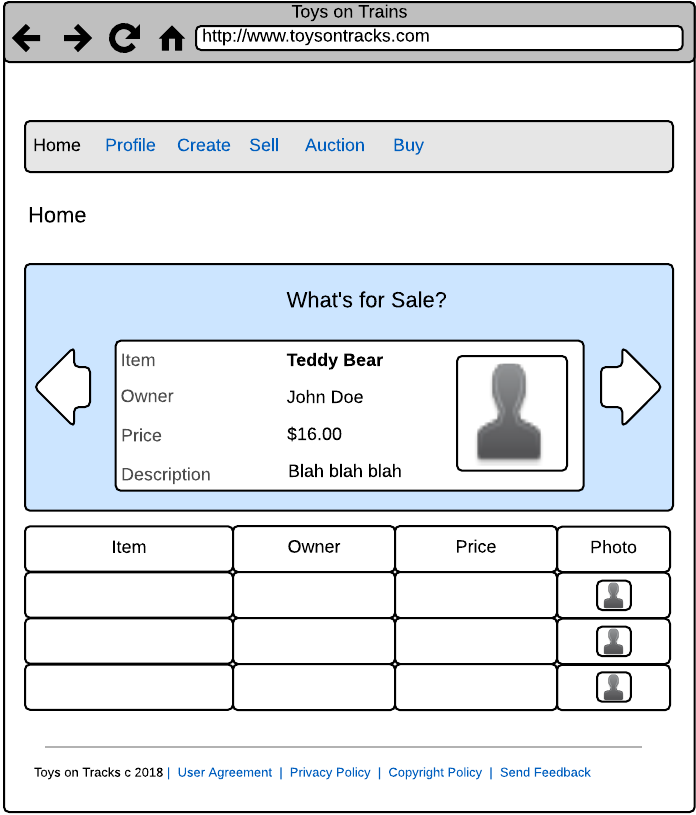
\includegraphics[height=6cm]{../img/home.png}

\caption{This is a wireframe of the home page.}

\end{figure}
\end{frame}

\begin{frame}{The Profile Page (Wireframe)}
\begin{figure} [!h]
    \centering
    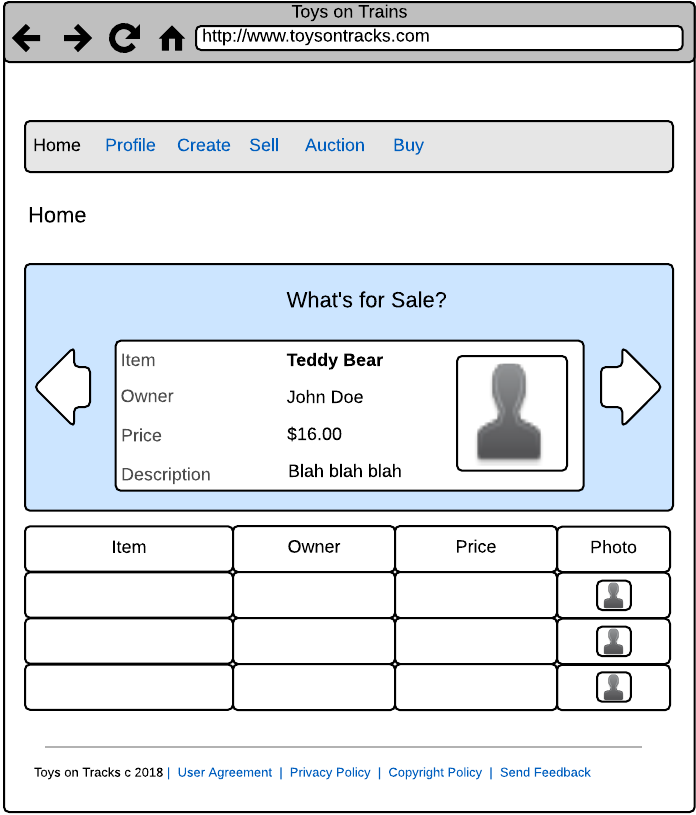
\includegraphics[height=6cm]{../img/home.png}

\caption{This is a wireframe of the profile page.}

\end{figure}
\end{frame}

\section{Implementation}

\begin{frame}{Rolling out the website}
\begin{itemize}
\item Tried to use a website generator to generate an example of a "working" website
\item That is, with Devise and other goodies installed.
\item Then make the final copy somewhere else.
\item Ended up using it as base for today's submissions.
\item Rails Composer broken
\item Any website involving Devise had errors 
\item Used prelang - abandonware from a year ago that got a Rails 4.x website
\end{itemize} 
\end{frame}


\begin{frame}[standout]
  Let's see the website at \url{https://limitless-escarpment-96871.herokuapp.com/}.
\end{frame}


\begin{frame}{What was implemented}
	\begin{itemize}
		\item A Ruby on Rails
		\item Uses Devise for Authentication
		\item Can be deployed to the cloud with minimum effort
	\end{itemize}
\end{frame}


\begin{frame}{What was NOT implemented}
	\begin{itemize}
		\item Code quality tools like Rspec
		\item APIs like Omniauth or Geocoding
		\item Allowing photos to be uploaded
	\begin{itemize}
		\item Could have been implemented easily in Development
		\item Need S3 to be implemented for Heroku
	\end{itemize}  
		\item Way of hidings the secret stuff in the YAML files.
		\item A website that came close to implementing the user stories.  
	\end{itemize}
\end{frame}


\section{Conclusion}

\begin{frame}{Comparisons with Django}
	\begin{itemize}
		\item Different terminology - same idea
	\begin{itemize}
		\item What is a "view" in Rails is a "template" in Django
		\item What is a "controller" in Rails is a "view" in Django
    \item Both share same concept of "models" and "URL routers"
	\end{itemize}  
		\item Easy to get started in Ruby on Rails than in Django
		\item Easy to find routes in Ruby on Rails than in Django
		\item Django has authentication built in (RoR needs Devise)
		\item Django's model migrations are far easier in 2018.
	\end{itemize}      
\end{frame}


\begin{frame}[standout]
  Questions?
\end{frame}

\appendix

\begin{frame}{About this presentation}

  This presentation was developed using \emph{Beamer}.

 \begin{center}\url{github.com/josephwright/beamer}\end{center}


  With the aid of the \emph{Metropolis} theme.

  \begin{center}\url{github.com/matze/mtheme}\end{center}


  The theme \emph{itself} is licensed under a
  \href{http://creativecommons.org/licenses/by-sa/4.0/}{Creative Commons
  Attribution-ShareAlike 4.0 International License}.

  \begin{center}\ccbysa\end{center}

\end{frame}


\end{document}
